%近畿大学理工学部情報学科卒業論文雛形兼論文作成の手引き
% ver 0.1 2005/11/28 by Toru Kato
% ver 0.2 2006/11/28 by Takashi Ishimizu
% ver 0.3 2007/11/26 by Toru Kato
% ver 0.4 2008/12/14 by Shoji Mizobuchi
% ver 0.5 2011/12/1 by Sen Moriya

\documentclass[12pt]{article}
\usepackage{luatexja}
\usepackage{luatexja-fontspec}
\usepackage{fontspec}
\usepackage{graphicx} % ← オプションなし!
\usepackage{amsmath}
\usepackage{eepic}
\usepackage{url}
\usepackage{booktabs}
\usepackage{caption}
\usepackage{listings}



\begin{document}
\pagestyle{empty}

\begin{center}
\vspace*{1cm}
\large
{\LARGE 卒業研究報告書}\\
\vspace*{0.8cm}
題目\\
\vspace*{1cm}
{\Huge \underline{スマートフォンを用いた持参薬識別支援システムの開発と有用性の検討}}\\
\vspace{3mm}
% {\LARGE \underline{副題があればここに書く}}\\

\vspace*{3cm}
指導教員\\
\vspace*{0.3cm}
\underline{\LARGE 森山 真光 准教授}\\
%\vspace*{-0.3cm}
%\underline{\hspace*{5cm}}\\
\vspace*{3cm}
報告者\\
\vspace*{0.3cm}

{22--1--211--0326}\\
\vspace*{0.3cm}
\underline{\Huge 久田 成真}\\
% \vspace*{-0.3cm}
% \underline{\hspace*{5cm}}\\
\vspace*{0.5cm}
近畿大学情報学部情報学科\\
\vspace*{2cm}
令和 07年 6月 11日提出\\
\end{center}

\newpage
\normalsize


%\tableofcontents
\clearpage
\begin{center}
{\bf \Large 概要}
\end{center} 

近年、入院患者が自身の常用薬を持参するケースが増加しており、臨床現場では薬剤の正確な識別が重要な課題となっている。特に高齢患者における多剤併用では、外観の似通った錠剤の識別が困難であり、薬剤師による目視確認には多大な時間と労力がかかる上、誤認のリスクも伴う。そこで本研究では、スマートフォンを用いた薬剤識別支援システムの有用性と実装可能性について検討した。

\begin{center}
  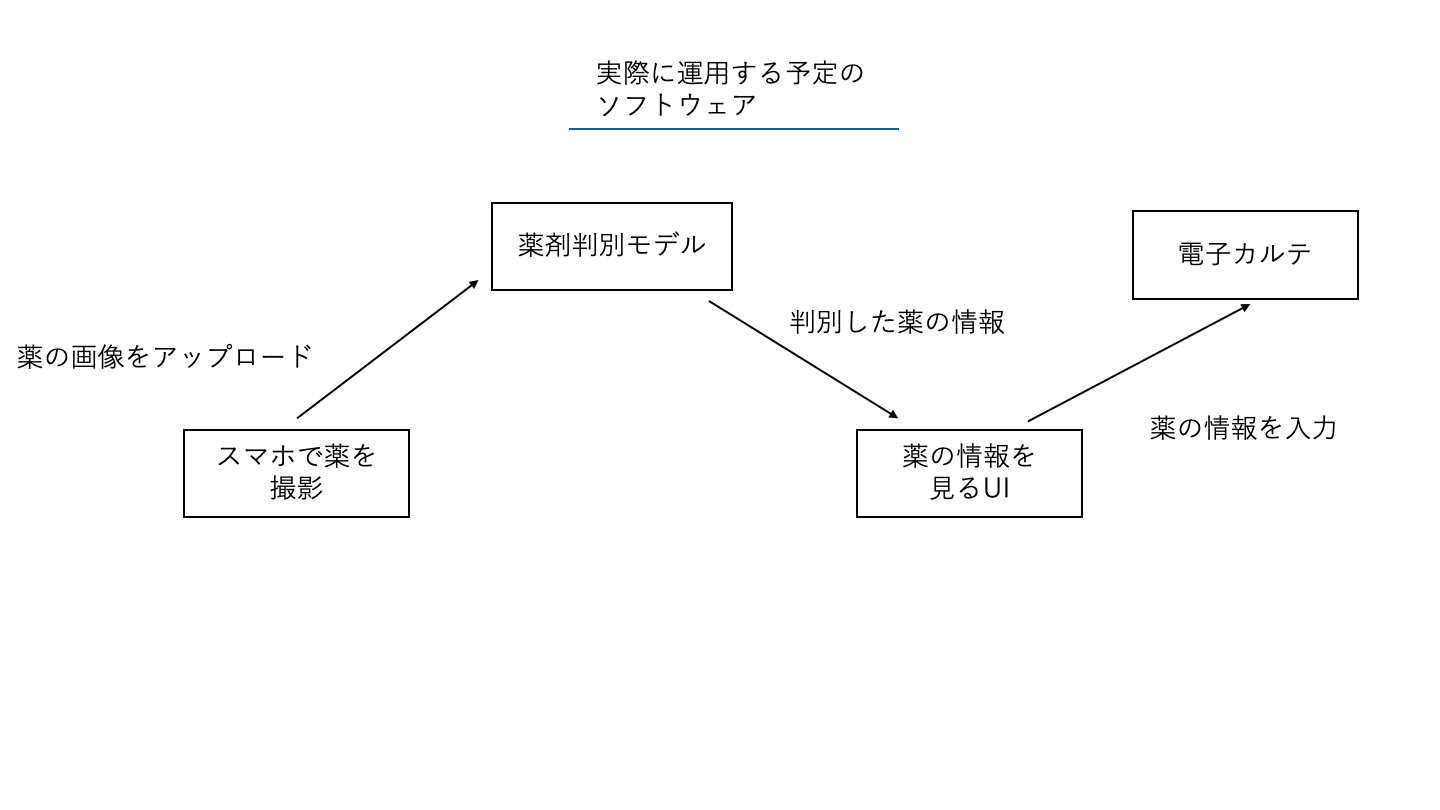
\includegraphics[width=13cm]{app_model_report.png}
\end{center}

\newpage

\tableofcontents
\newpage
\setcounter{page}{1}
\pagestyle{plain}

\section{序論}\label{sec1}
\subsection{本研究の背景}
現代の医療現場では、入院患者が自宅で服用していた常用薬を持参することが一般的となっている。特に高齢者においては、複数の薬剤を併用する「多剤併用(ポリファーマシー)」のケースが多く、患者が持参する薬の種類や形状、色は多岐にわたる。その結果、医療従事者、とりわけ薬剤師が病室で持参薬を確認・識別する作業は、非常に煩雑かつ時間を要するプロセスとなっている。また、薬剤の外観が似通っていることや、患者の誤った申告、薬の包装やラベルの欠損といった状況も重なり、正確な薬剤識別が困難になることが少なくない。

このような状況下で誤認識が生じれば、薬剤の重複投与や相互作用による副作用といった重大な医療事故につながる可能性がある。そのため、持参薬の正確かつ迅速な識別は、患者の安全確保と医療の質の向上に直結する重要な課題である。

従来、薬剤師は目視による確認や製薬会社が提供する薬剤写真をもとに照合を行っていたが、これらは人手と時間に依存しており、効率性と信頼性の両面で限界がある。こうした背景を踏まえ、近年では、ICTやAIを活用して薬剤識別を支援するシステムの開発が注目されている。特に、スマートフォンの高性能化と機械学習技術の進展により、医療現場での画像認識技術の応用が現実的な選択肢となってきている。

本研究では、こうした課題の解決を目的に、スマートフォンを用いた錠剤識別支援システムの構築を目指す。深層学習をベースとした画像認識技術を活用することで、薬剤師が病室で素早く正確に錠剤を判別できる環境を整備し、薬剤誤投与のリスクを低減するとともに、業務の効率化を図ることを目指す。


\subsection{本研究の目的}
本研究の目的は、病院における持参薬の識別作業を効率化し、薬剤師の業務負担軽減と薬剤誤投与の防止を実現することである。特に多剤併用の患者を対象とし、外観が似通った複数の錠剤を迅速かつ正確に識別するため、スマートフォンを用いた画像認識技術による薬剤識別支援システムの構築を目指す。深層学習モデルを用いて錠剤を自動検出・分類し、持参薬の確認作業を支援することで、臨床現場における安全性と効率性の向上に貢献することを目的とする。
\subsection{本報告書の構成}

\newpage

\section{関連研究}\label{sec2}
Dangらの研究\cite{Dang_2024}では、視覚障害のある人々がスマートフォンのカメラを使用して錠剤を識別できるようにアプリを作っている。
その中で、薬の錠剤を識別するシステムを設計している。
このアプリケーションでは、YOLO(You Only Look Once)というオブジェクト検出モデルの最新版であるYOLOv8フレームワークが活用されている。YOLOは、入力画像を処理して特徴を抽出し、それをグリッドに分割することで、各セルでオブジェクトの有無を効率的に予測することができる。

モデルのトレーニングには、アメリカ国立医学図書館が管理するPillboxデータセットが使用されている。このデータセットには、米国内で販売されている錠剤の写真8,693枚が含まれており、それぞれに形状、色、刻印、サイズ、有効成分、製造元といった詳細な薬剤情報が付随している。こうした情報は、さまざまな種類の錠剤の形状や識別の違いを認識するために不可欠である。

さらに、YOLOv8のアーキテクチャは錠剤検出に特化するように変更されており、錠剤固有の特徴をより正確に捉えられるようカスタマイズされている。特に、畳み込み層は錠剤の形状や刻印の微細な違いを検出できるようにファインチューニングされており、これがバウンディングボックスの精度や錠剤の分類精度を高めている。現在、このモデルは32種類の異なる錠剤カテゴリを予測可能であり、平均平均精度(mAP)99.5\%という高い精度で錠剤の検出と識別を実現している。

Kwonらの研究では、\cite{chemosensors10010004}限られた学習データで医薬品検査のための錠剤検出性能を向上させるディープラーニングアルゴリズムを提案している。複数の錠剤が写った画像において個々の錠剤を検出する際、錠剤の種類が増加すると画像中の錠剤の組み合わせが指数関数的に増え、学習データの取得およびラベル付けの作業が複雑になる。この問題に対処するため、本研究では単一の錠剤画像のみを学習データとして使用する手法を提案している。

提案手法では、Mask R-CNNに基づく2段階の検出プロセスを採用している。第1段階では、錠剤の種類に関係なく画像中の錠剤の数と領域(エリア)を検出する。この学習には、複数の錠剤が写った画像を使用している。第2段階では、第1段階で検出された錠剤を背景から分離し、対応する錠剤の種類を検出する。この段階では、単一錠剤画像を学習に用いている。

また、第1段階で得られた錠剤領域検出モデルを用いて、単一錠剤画像に対するデータラベリングを自動化し、JSONファイルを生成する手法も提案している。これにより、学習データの準備にかかる時間と労力の削減が可能となる。

さらに、学習中のデータ不足を補うために、露光や回転によるデータ拡張を行っている。加えて、隣接する錠剤による誤検出や非検出、特定の角度での検出失敗といった問題を解決するために、後処理アルゴリズムを適用している。これには、領域の拡張、複数の検出結果からの最大領域の選択、非検出時の段階的な回転検出などが含まれる。

実験の結果、提案手法は限定的な画像枚数と小規模なデータセットにもかかわらず、既存のアルゴリズムと比較して高い検出性能を示した。特に、後処理アルゴリズムの適用によって、精度および正答率が向上した。また、白色錠剤の側面画像に対するデータ収集条件の追加も検出性能の向上に寄与している。YOLOv3との比較では、提案手法の方が正答率が高い結果を得ている。

この手法は、自動薬剤払い出し機などの自動装置の性能向上に貢献し、払い出された錠剤の検査において生産性の損失やヒューマンエラーを最小限に抑えることが期待される。今後の課題としては、さまざまな環境下での実験の実施や、最新のTransformerベース技術の応用が挙げられている。

\bibliographystyle{plain}  % スタイル(plain, unsrt, alpha など)
\bibliography{refs}        % refs.bib を参照(拡張子は書かない)

\end{document}
 

%%% Local Variables: 
%%% mode: latex
%%% TeX-master: t
%%% End: 